\section{Konrad Małek}
\label{sec:konradmalek}

\subsection*{F1 car}

\label{sub:f1}


\textbf{Formula 1 car} (see Figure~\ref{fig:bolid}) is a single-seat racing car with an open body and wheels protruding outside the cockpit profile, built according to \textbf{FIA Formula 1 regulations }. Its specifications have changed over the years. The cost of designing and building a racing car requires hundreds of hours in the wind tunnel, and costs often exceed \underline{\$100 million.}\par
The aerodynamic elements of cars are designed to obtain the best possible downforce (reduced wheel slip and increased power efficiency from the wheels on the ground) at the highest possible speed and acceleration. The last part is designed with this in mind. Early Formula 1 cars used streamlined applications, without the characteristic aerodynamics-enhancing elements (\textit{spoilers}), which were soon launched by the initial downforce-improving bases and Formula 1 cars, distinguished by extended front and front mechanisms.

\vspace{5mm}
\begin{figure}[h] 
    \centering
    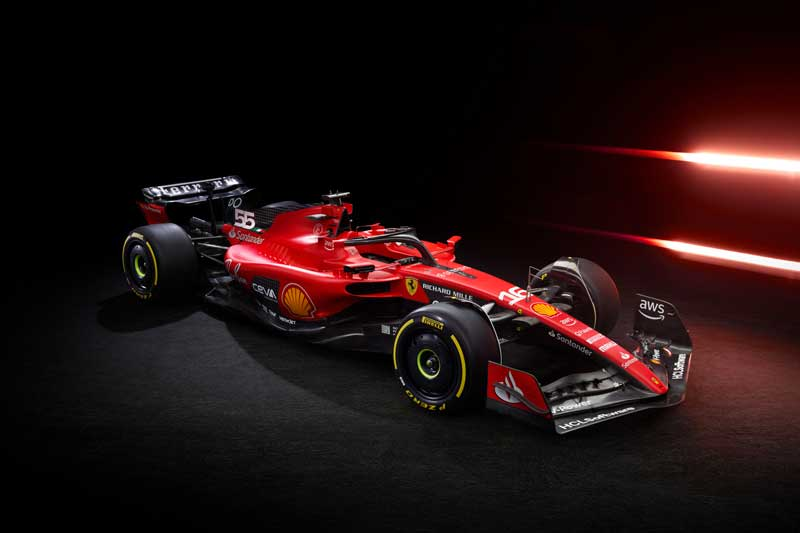
\includegraphics[width=0.9\textwidth]{pictures/bolid_f1.jpg} 
    \caption{Scuderia Ferrari's F1 car }
    \label{fig:bolid}
\end{figure}

\newpage
\subsection*{The most important elements of an F1 car}
\label{sub:elementy}

\begin{enumerate}
    \item Engine  
    \begin{itemize}
        \item[$\spadesuit$] V6 - currently using (see Figure~\ref{fig:silnik})
        \item[$\spadesuit$] v8 
        \item[$\spadesuit$] v10
        
    \end{itemize}
    \item Gearbox (semi-automatic)
    \item Construction
    \item Tires (see Figure~\ref{fig:opony}), in which we distinguish:\begin{itemize}
        \item Soft
        \item Medium
        \item Hard 
    \end{itemize}
    \item Brakes
    \item Halo - driver protection system
\end{enumerate}





\begin{figure}[h]
\begin{center}
\begin{minipage}[b]{6cm}
\centering
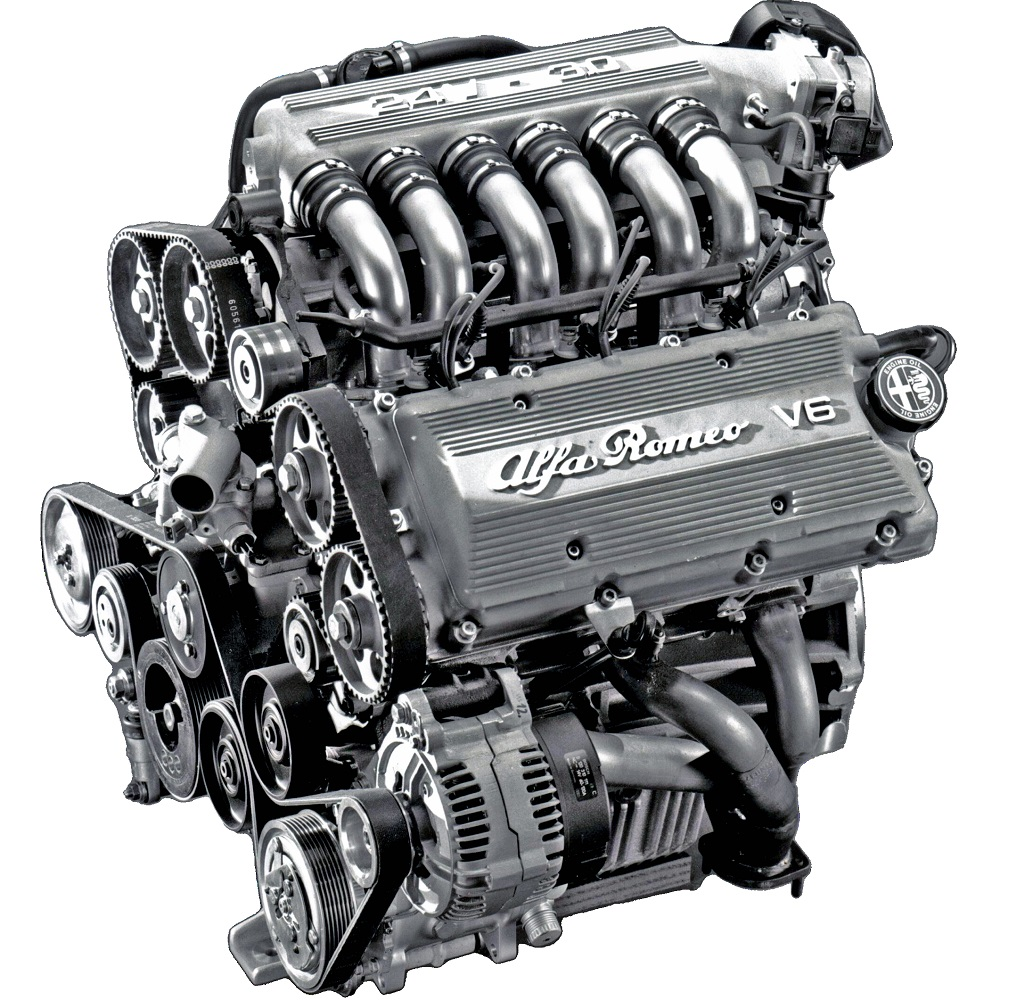
\includegraphics[width=0.7\textwidth]{pictures/v6.jpg} 
\caption{Engine V6}
\label{fig:silnik}
\end{minipage}
\begin{minipage}[b]{6cm}
\centering
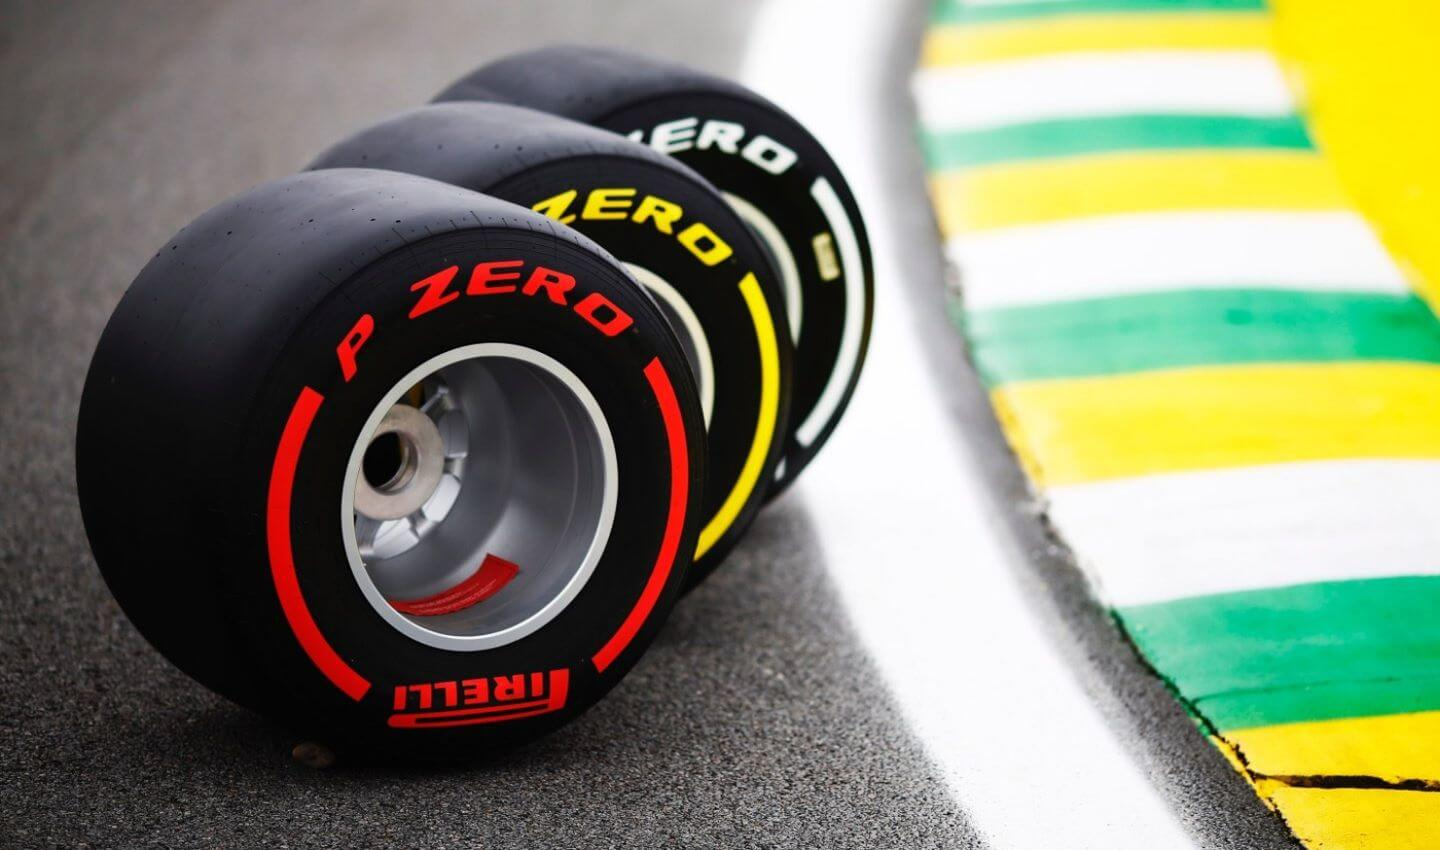
\includegraphics[width=0.7\textwidth]{pictures/opony.jpg} 
\caption{Pirelli's tires}
\label{fig:opony}
\end{minipage}
\end{center}
\end{figure}




\subsection*{Equations:}
\begin{equation}
\label{eq:calka1}
\int (\alpha f(x) + \beta g(x)) dx = \alpha \int f(x) dx + \beta \int g(x) dx
\end{equation}
\begin{equation}
\label{eq:granica1}
\lim_{\Delta x \to 0} \frac{f(x_{0} + \Delta x) - f(x_{0})}{\Delta x} = f'(x_{0})
\end{equation}

\newpage
\subsection*{Table presents current F1 results}

\begin{table}[h]
\centering
\begin{tabular}{|llccc|}
\hline
\multicolumn{5}{|c|}{Driver Classification}                                                                                                            \\ \hline
\multicolumn{2}{|c|}{Driver}                                  & \multicolumn{1}{c|}{Country} & \multicolumn{1}{c|}{Team}          & Points \\ \hline
\multicolumn{1}{|l|}{1.} & \multicolumn{1}{l|}{Max Verstappen}  & \multicolumn{1}{c|}{Netherlands}         & \multicolumn{1}{c|}{Red Bull Racing} & 466    \\ \hline
\multicolumn{1}{|l|}{2.} & \multicolumn{1}{l|}{Sergio Perez}    & \multicolumn{1}{c|}{Mexico}           & \multicolumn{1}{c|}{Red Bull Racing} & 240    \\ \hline
\multicolumn{1}{|l|}{3.} & \multicolumn{1}{l|}{Lewis Hamilton}  & \multicolumn{1}{c|}{Great Britain}  & \multicolumn{1}{c|}{Mercedes}        & 201    \\ \hline
\multicolumn{1}{|l|}{4.} & \multicolumn{1}{l|}{Fernando Alonso} & \multicolumn{1}{c|}{Spain}        & \multicolumn{1}{c|}{Aston Martin}    & 183    \\ \hline
\multicolumn{1}{|l|}{5.} & \multicolumn{1}{l|}{Carlos Sainz}    & \multicolumn{1}{c|}{Spain}        & \multicolumn{1}{c|}{Ferrari}         & 173    \\ \hline
\end{tabular}
\label{tab1:klasyfikacja}
\caption{The first five F1 drivers as of October 27, 2023}
\end{table}
